\subsection{Detailed design}
\subsubsection{Diagrams}
\begin{figure}
\centering
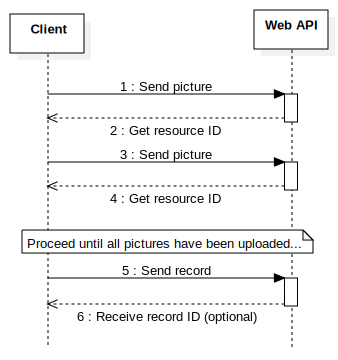
\includegraphics[scale=0.75]{server/SequenceDiagram-AddRecord.svg}
\caption{Sequence diagram: adding a record through the web API}
\label{fig:addRecordSequenceDiagram}
\end{figure}
\subsubsection{Significant data structures}

The web API is going to make use of the Record and Specimen data structures,
which will be exchanged between the server and its clients (the Android
application and the website). They will be represented in a JSON format, which 
is readily available for use in PHP, JavaScript, and Android. Data types, where
specified, are JSON data types.

The structure of a Record is as follows:
\begin {verbatim}
Record : Object
    UserName : String
    UserPhone : String
    LocationName : String 
    Specimens : Array of Specimen
\end {verbatim}

The structure of a Specimen is as follows:
\begin {verbatim}
Specimen : Object
    SpeciesName : String
    LocationLatitude : Number
    LocationLongtitude : Number
    Abundance : Number
    Comment : String
    ScenePhoto : String (ID of a resource on the server)
    SpecimenPhoto : String (ID of a resource on the server)
\end {verbatim}

The web API is going to use a relational database as a data store.
The database tables are as follows:

\begin {verbatim}
Users
    UserId : INT auto-increment PK
    UserName : VARCHAR(20) not-null
    UserFullName : VARCHAR(50)
    UserPhone : VARCHAR(20)
    UserEmail : VARCHAR(50)
    UserPassword : BINARY(20)
    
Records
    RecordId : INT auto-increment PK
    UserId : INT not-null
    LocationName : VARCHAR(50)
    
Specimens
    SpecimenId : INT auto-increment PK
    RecordId : INT not-null
    SpeciesName : VARCHAR(255) not-null
    Latitude : FLOAT(10,6)
    Longitude : FLOAT(10,6)
    Abundance : INT
    Comment : TEXT
    ScenePhoto : INT
    SpecimenPhoto : INT   
\end {verbatim}